% Este documento se realizó con el propósito de proporcionale a los estudiantes
% del CIDETEC un machote en latex de la tesis. Espero que les sirva de ayuda.
% Atte: Dr. Miguel Gabriel Villarreal Cervantes.
%*****************************************************************************
%*****************************************************************************
% Capítulo I
\chapter{Introducción \label{cap1}}

Como nos ha marcado la experiencia la computadora al igual que cualquier otra
 máquina fue diseñada para facilitar la vida de las personas, ya sea acelerando
 o automatizando tareas, así mismo se ha llegado a un punto en la operación de
 la computadora en la que se realizan tareas de forma mecanizada ya se repiten
 frecuentemente y no hay variantes en estas.  

Los desarrolladores de software han contribuido a la automatización de estas
 tareas, sin embargo, cuando es software no es especifico para una persona sino
 para un grupo de personas, las acciones llegan a ser tan variadas de un usuario
 a otro que el desarrollador no puede prever el comportamiento de todos los
 usuarios en el ambiente desarrollado. 

En el estado del arte se presentan algunos desarrollos que van enfocados a la
 automatización de acciones humanas, con las variantes que estas involucran en
 el mundo real. La mayoría de estos desarrollos van enfocados a la robótica,
 sin embargo, la solución también puede ser enfocada a un ambiente virtual.  

La propuesta aquí presentada va enfocada al apoyo de las personas con acceso a
 la computadora, por su situación laboral, pero que debido a sus capacidades
 físicas no puede usar el equipo con la misma agilidad que una persona con
 todas sus facultades. Estas son las Personas con Movilidad Reducida(PRM), que
 principalmente, por cuestiones laborales tienen que trabar con una computadora
 y que por su discapacidad se les dificulte el uso de la misma.

Por lo tanto en este trabajo de investigación se propone, como un sistema que
 va a monitorear las acciones que el usuario realiza con los dispositivos de
 E/S (ratón y teclado) y  descubrir las acciones frecuentes para posteriormente
 reproducirlas de la misma forma que lo haría el usuario.

\section{Estado del arte}
En esta sección se mostraran los trabajos relacionados o similares al proyecto
 propuesto en este documento y una breve descripción de estos. En la
 investigación realizada se han encontrado trabajos cuyo objetivo es obtener
 que un robot mecánico o virtual realice tareas de manera similar a como las
 haría un humano. 


Los archivos por lotes (Batch o Script Shell) \cite{Silberschatz1999} son
 archivos que contienen instrucciones para el sistema operativo en formato
 ASCII por lo que son dependientes de él, por lo general tienen la extensión
 .bat o .sh, sin embargo, para el caso de UNIX esto no es obligatorio. En la
 imagen ~\ref{fig:script} se muestra el codigo de un archivo por lotes y la 
 ejecucion en consola.


\begin{figure}[H]
\centering
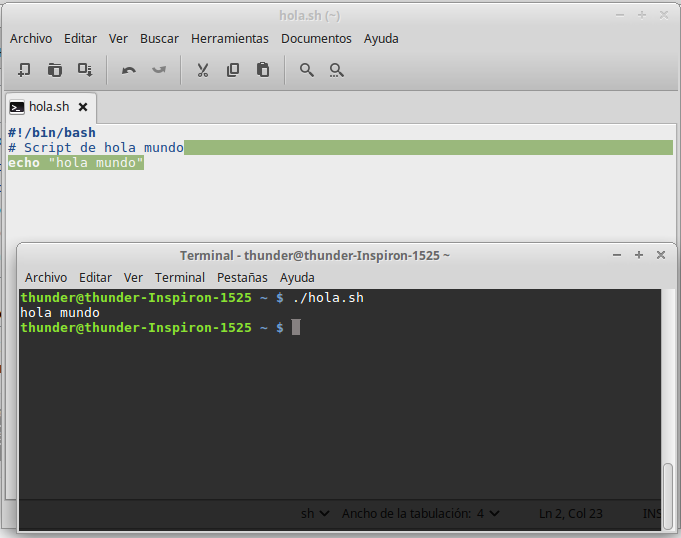
\includegraphics[width=0.5\columnwidth]{CapituloI/Imagenes/Script.png}
\caption{Ejemplo de un archivo por lotes para Linux.}
\label{fig:script}
\end{figure}


Pulover's Macro Creator\cite{Batista}, desarrollado y mantenido principalmente
 por Rodolfo U. Batista, es una herramienta de automatización y creación de
 scripts basada en el lenguaje "AutoHotKey". Este  creador de macros facilita
 la tarea de la creación del script por medio de  su interfaz grafica o con la
 grabadora de macros que proporciona. Entre sus características, este el
 proporcionar  control de ventanas en segundo plano y sentencias de
 control(ciclos y condicionales). En la imagen ~\ref{fig:macros} se puede observar la interfaz de usuario del software.


\begin{figure}[H]
\centering
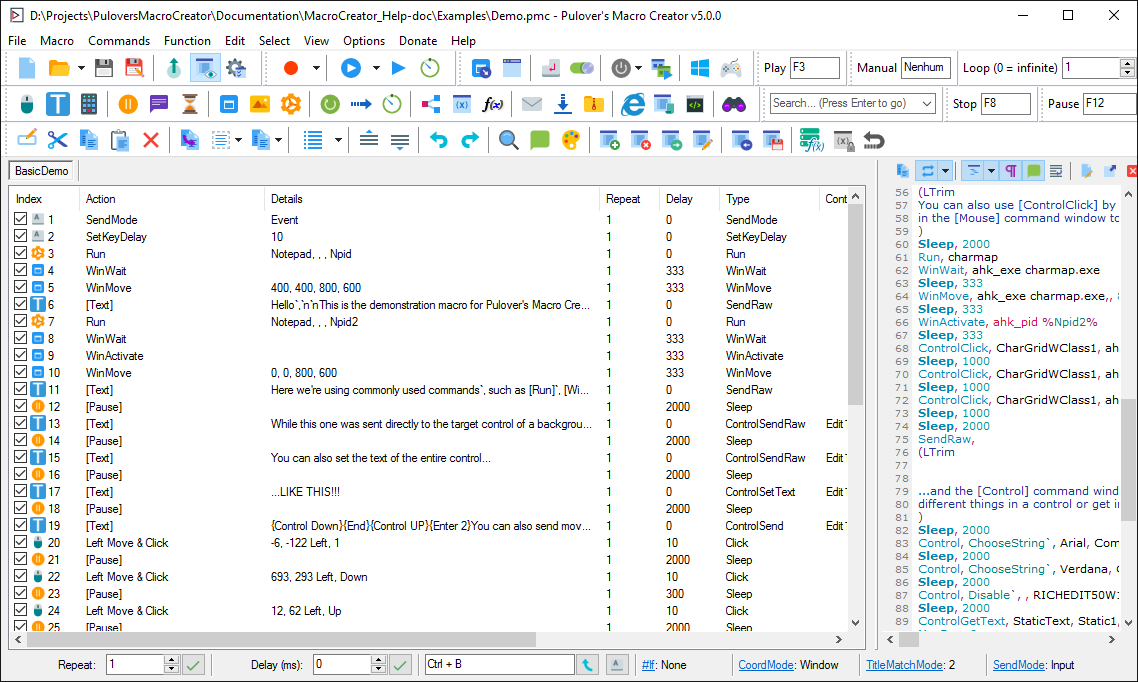
\includegraphics[width=0.5\columnwidth]{CapituloI/Imagenes/Macros.png}
\caption{Interfaz de usuario de Pulover's Macro Creator con una mmacro de
 ejemplo.}
\label{fig:macros}
\end{figure}



Un trabajo desarrollado por la Universidad de Tsukuba en
 Japón\cite{Nakano2006}, tiene por objetivo el crear un oponente virtual
 al nivel de un oponente humano que represente un reto para el jugador. Para
 lograr esto se crearon perfiles con las estrategias de los jugadores y
 posteriormente se reproducen en otra partida, en la imagen ~\ref{fig:imitat}
 se muestra el entorno del juego.


\begin{figure}[H]
\centering
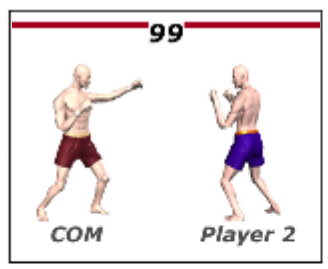
\includegraphics[width=0.5\columnwidth]{CapituloI/Imagenes/Imitating.png}
\caption{Ambiente del juego de accion.}
\label{fig:imitat}
\end{figure}


En el trabajo desarrollado en la Universidad Tecnológica de Lanzhou en China
 \cite{Zhang2017},hacen un análisis del comportamiento del soldador experto
 humano utilizando un sistema de inferencia neurodifuso adaptativo (ANFIS,
 por sus siglas en ingles) para su automatización, considerando las variables
 de los materiales usados y caracterizando la tarea del soldador humano.
 En la imagen ~\ref{fig:syswelding} se puede apreciar el sistema experimental resultante del proyecto mencionado.


\begin{figure}[H]
\centering
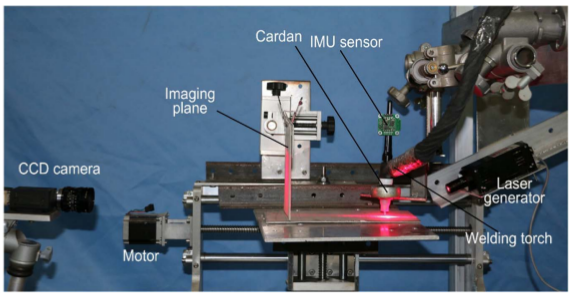
\includegraphics[width=0.8\columnwidth]{CapituloI/Imagenes/Welding.png}
\caption{Sistema experimental de la soldadora.}
\label{fig:syswelding}
\end{figure} 
 

En el ambiente artístico \cite{Nishiguchi2017}, el trabajo desarrollado en
 Japón por la Universidad de artes de Tokyo y la Universidad de Osaka, cuyo
 objetivo era brindar un comportamiento natural humano a un Robot Humanoide.
 Para cumplir esto utilizaron el conocimiento del director de escena Hirata,
 que dada la precisión en sus instrucciones a los actores, facilita la
 traducción de esas órdenes a las reglas para el robot humanoide, además,
 desarrollaron una interfaz de usuario para que el manejo del robot sea más
 sencillo, ayudando a los principiantes, ya que proporcionan menos datos se
 puede obtener buenos resultados. Como se puede observar en la imagen
 ~ref{fig:theatricalrob} el robot llego a desempeñar un amigo del
 personaje principal en la obra "Night on the milky way train" en un ecenario
 real.


\begin{figure}[H]
\centering
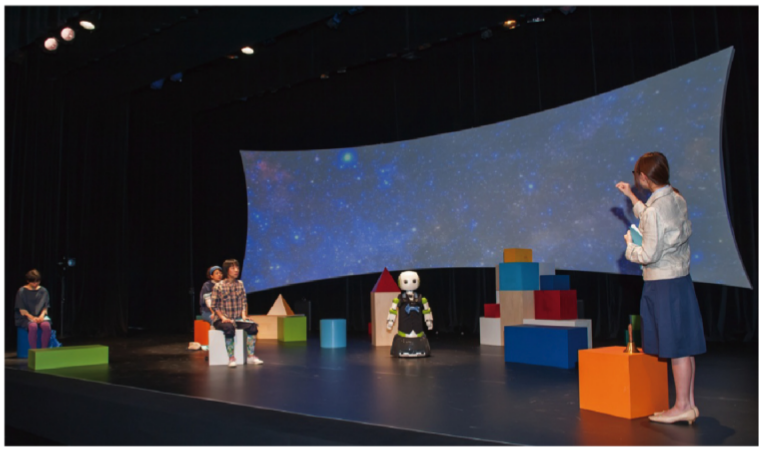
\includegraphics[width=0.8\columnwidth]{CapituloI/Imagenes/Theatrical.png}
\caption{Robot humanoide actor en ecenario real.}
\label{fig:theatricalrob}
\end{figure} 


El trabajo desarrollado por la Universidad de Plymouth, Universidad de Lincoln
 ambas en el Reino Unido y la Universidad de Gante en Bélgica\cite{Senft2016},
 realiza la comparativa de su método SPARC (Supervised Progressively Autonomous
 Robot Competencies) con el IRL (Interactive Reinforcement Learning), estos dos
 métodos se basan en el aprendizaje automático de un robot, haciendo que un
 humano con conocimiento del tema de la aprobación de la actividad que está
 realizando o que va a realizar el robot. Ambos sistemas fueron probados en un
 ambiente virtual nombrado “sophie’s kitchen”, el cual se puede apreciar en la
 imagen ~\ref{fig:sparcrob}, con objetivo es hornear un pastel.
 
 
\begin{figure}[H]
\centering
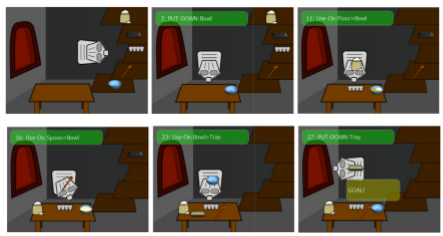
\includegraphics[width=0.8\columnwidth]{CapituloI/Imagenes/Sparc.png}
\caption{Robot virtual en “sophie’s kitchen”.}
\label{fig:sparcrob}
\end{figure}


El trabajo realizado en la Universidad Nacional Chiao Tung y el Instituto
 Politécnico Kaohsiung ambos en Taiwán\cite{Chang1996}, propone un algoritmo
 que imite el comportamiento del aprendizaje humano como una solución al
 aprendizaje automático en ambientes imperfectos, por ejemplo, cuando la
 información esta incompleta. Este algoritmo demuestra en los experimentos
 realizados, ser superior al ID3 y PRISM.


\section{Justificación}
A nivel mundial, la discapacidad va en aumento dado que la población está
 envejeciendo y son pocos los programas privados y gubernamentales que apoyan a
 este grupo de personas\cite{OrganizacionMundialdelaSalud2011}. 
 Con referencia a los datos obtenidos del Censo de Población
 y Vivienda de 2010 era poco más del 5\% de la Población de México la que
 presentaba algún tipo de discapacidad, pero se puede apreciar que esta cifra va
 en aumento ya que en la Encuesta Nacional de Ingresos y Gasto de los Hogares
 (ENIGH) de 2012 fue el 6.6\% el porcentaje de la población la que tenía alguna
 discapacidad\cite{Milosavljevic2014}.
 

%Falta Escribir

 
La Organización Mundial de la Salud (OMS) y el Banco Mundial
\cite{OrganizacionMundialdelaSalud2011} proponen una
 estrategia de colaboración entre el sector privado y gubernamental para
 rehabilitar e incorporar a la sociedad a las personas discapacitadas y así
 poder aprovechar el potencial de toda esta gente.Algunas de estas propuestas
 tienen por objetivo proporcionar accesibilidad en los servicios convencionales
 , por ejemplo transporte y educación, así como adiestrar a los servidores
 públicos, para que las personas sean tratadas con los cuidados necesarios.
 
 
Como un apoyo a las personas que por su discapacidad presentan dificultad para
 interactuar de manera ágil y precisa con las computadoras de escritorio, se
 plantea desarrollar un sistema de reconocimiento de patrones con la capacidad
 reproducir las acciones que tengan mayor incidencia de uso.

\section{Planteamiento del problema}
Con base en lo mencionado previamente, se puede apreciar que la población de
 Personas con Movilidad Reducida(PRM) va en aumento en México y con el uso de
 la computadora como algo imprescindible en la actualidad sobre todo en el
 sector laboral 2, la discapacidad de estas personas puede representar un
 obstáculo en su desarrollo laboral.



\section{Objetivo general} 
Diseñar y desarrollar un software que defina a partir de un periodo de tiempo
 determinado el conjunto de acciones con mayor incidencia de uso por un usuario
 realizadas en una computadora por un usuario, para su uso posterior.

\section{Objetivos específicos}
\begin{itemize}
  \item Desarrollar del sistema para la captura de acciones, tanto del  ratón
  como del teclado.
  \item Obtener una muestra de las acciones realizadas con el teclado y el 
  ratón por un usuario en una computadora.
  \item Diseñar y desarrollar el algoritmo para la determinación de tareas
  repetitivas.
\end{itemize}


\section{Metodología}
Con el propósito de desarrollar y lograr los objetivos propuestos en el presente trabajo de investigación, se plantearon siguientes metas:
\section*{Metas}
\begin{itemize}
  \item[I] Investigación de sistemas similares.
  \item[II] Recopilación de resultados de sistemas similares.
  \item[III] Desarrollo del sistema  de captura de datos.
  \item[IV] Obtención de los datos de ejemplo.
  \item[V] Desarrollo del Sistema de procesamiento de datos.
  \item[VI] Realizar pruebas del sistema.
  \item[VII] Realizar comparativa de los resultados.
\end{itemize}





\section{Cronograma de actividades}

\begin{figure}[h]
\centering
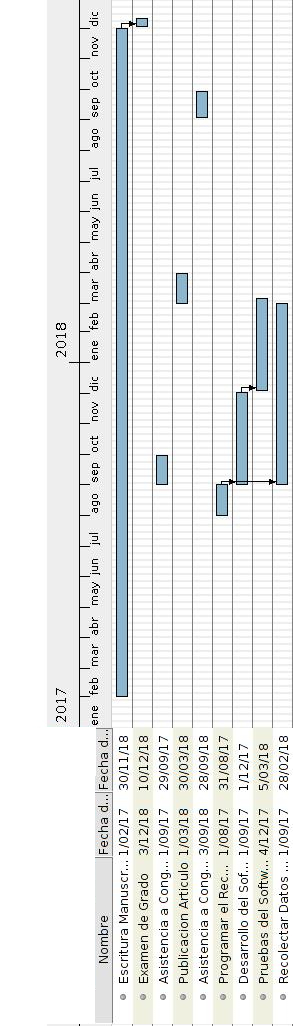
\includegraphics[width=0.3\columnwidth]{./CapituloI/Imagenes/Cronograma.jpg}
\end{figure}


